% This LaTeX document needs to be compiled with XeLaTeX.
\documentclass[
  10
]{article}
\usepackage[margin=2cm,includehead=true,includefoot=true,centering,]{geometry}
\usepackage{xcolor}
\usepackage{ucharclasses}
\usepackage{hyperref}
\usepackage{amsmath,amssymb}
\usepackage{amsfonts}
\usepackage[version=4]{mhchem}
\usepackage{stmaryrd}
\usepackage{bbold}
\usepackage{fontspec}
\usepackage{ctex}
\usepackage[export]{adjustbox}
\usepackage{tabularx}
\usepackage{booktabs}

\usepackage{setspace}
\setstretch{1.2}

\makeatletter
\@ifundefined{KOMAClassName}{% if non-KOMA class
  \IfFileExists{parskip.sty}{%
    \usepackage{parskip}
  }{% else
    \setlength{\parindent}{0pt}
    \setlength{\parskip}{6pt plus 2pt minus 1pt}}
}{% if KOMA class
  \KOMAoptions{parskip=half}}
\makeatother
\usepackage{longtable,booktabs,array}
\newcounter{none} % for unnumbered tables
\usepackage{multirow}
\usepackage{calc} % for calculating minipage widths
% Correct order of tables after \paragraph or \subparagraph
\usepackage{etoolbox}
\makeatletter
\patchcmd\longtable{\par}{\if@noskipsec\mbox{}\fi\par}{}{}
\makeatother
% Allow footnotes in longtable head/foot
\IfFileExists{footnotehyper.sty}{\usepackage{footnotehyper}}{\usepackage{footnote}}
\makesavenoteenv{longtable}
\usepackage{graphicx}
\makeatletter
\newsavebox\pandoc@box
\newcommand*\pandocbounded[1]{% scales image to fit in text height/width
  \sbox\pandoc@box{#1}%
  \Gscale@div\@tempa{\textheight}{\dimexpr\ht\pandoc@box+\dp\pandoc@box\relax}%
  \Gscale@div\@tempb{\linewidth}{\wd\pandoc@box}%
  \ifdim\@tempb\p@<\@tempa\p@\let\@tempa\@tempb\fi% select the smaller of both
  \ifdim\@tempa\p@<\p@\scalebox{\@tempa}{\usebox\pandoc@box}%
  \else\usebox{\pandoc@box}%
  \fi%
}
% Set default figure placement to htbp
\def\fps@figure{htbp}
\makeatother
\setlength{\emergencystretch}{3em} % prevent overfull lines
\providecommand{\tightlist}{%
  \setlength{\itemsep}{0pt}\setlength{\parskip}{0pt}}


\hypersetup{colorlinks=true, linkcolor=blue, filecolor=magenta, urlcolor=cyan,}
\urlstyle{same}

\usepackage{colortbl}
\definecolor{table-row-color}{HTML}{999999}
\definecolor{table-rule-color}{HTML}{999999}
%\arrayrulecolor{black!40}
\arrayrulecolor{table-rule-color}     % color of \toprule, \midrule, \bottomrule
\setlength{\aboverulesep}{0pt}
\setlength{\belowrulesep}{0pt}


% Font selection handled by ctex package


\author{}
\date{}

\begin{document}


\section{小而强大：利用轻量级大语言模型增强时序预测}
\label{small-but-mighty-enhancing-time-series-forecasting-with-lightweight-llms}

范浩然$^{1}$, 李斌$^{2\dagger}$, 翁逸轩$^{3}$, 周守军$^{2}$

$^{1}$ 重庆邮电大学计算机科学与技术学院，重庆南岸区，400065，中国

$^{2}$ 中国科学院深圳先进技术研究院，深圳南山区，518055，中国

$^{3}$ 西湖大学，杭州西湖区，浙江，310024，中国

通讯作者邮箱: 2022212169@stu.cqupt.edu.cn; b.li2@siat.ac.cn;
sj.zhou@siat.ac.cn; wengsyx@gmail.com; $\dagger$通讯作者

\subsection{摘要}\label{abstract}

虽然大语言模型（LLMs）在时序预测中展现出巨大潜力，但其实际部署仍受到过大计算需求和
内存占用的制约。现有的基于LLM的方法通常面临三个关键局限：（1）处理数值化时序模式时
参数利用效率低下；（2）连续时间信号与离散文本嵌入之间存在模态不一致；（3）难以灵活
集成实时专家知识。本文提出\textbf{SMETimes}（Small but Mighty Enhancing Time Series），
首次系统性地研究了参数规模在30亿以下的小语言模型（SLM）用于高效、准确的时序预测。
我们的方法聚焦于三项核心创新：（1）一种\textbf{统计增强的提示结构}，通过描述性统计
特征将数值型时序与文本语义连接起来；（2）一种\textbf{自适应融合嵌入结构}，通过可学习
参数对齐时序模式与语言模型的token空间；（3）一种\textbf{动态混合专家（MoE）结构}，
借助SLM的计算效率，自适应地融合基础预测与领域专用模型。在七个基准数据集（ETTh1/2、
ETTm1/2、Weather、Solar、ECL）上的广泛评估表明，我们30亿参数的SLM在五个主要数据集
上达到了最先进的性能，同时训练速度比70亿参数LLM基线快\textbf{3.8倍}，内存占用降低
\textbf{5.2倍}。特别地，所提模型展现出较强的学习能力，MSE比传统LLM低\textbf{12.3\%}。
消融实验验证了统计增强的提示结构和自适应融合嵌入结构分别在长时段预测任务中贡献了
\textbf{15.7\%}和\textbf{18.2\%}的误差降低。本研究重新定义了效率-精度的权衡格局，
确立了SLM作为资源密集型LLM在实用时序预测中的可行替代方案。代码和模型已开源：
https://github.com/xiyan1234567/SMETimes。

关键词：小语言模型，统计增强提示，自适应融合嵌入，动态混合专家

\subsection{1 引言}\label{introduction}

时序预测是现代决策系统的基石，广泛应用于能源管理{[}30{]}、金融市场{[}42{]}、
气候建模{[}1{]}和智能交通{[}23{]}等关键领域。传统方法通常依赖领域专用的
统计模型{[}2{]}或深度神经网络{[}3{]}，需要大量计算资源和广泛的领域知识。
尽管大语言模型（LLMs）最近在时序预测中展现出了令人瞩目的能力{[}4, 21{]}，
但其实际部署面临着由于过高的计算成本和内存占用带来的重大挑战{[}5{]}。

近年来基于LLM的预测方法{[}6, 7{]}的涌现揭示了三个根本性局限：
（1）海量参数（通常\textgreater7B）导致训练和推理效率低下；
（2）数值时序模式与文本嵌入之间对齐不足；
（3）集成领域专用专家知识的灵活性有限。如图1所示，传统LLM方法如
Time-LLM{[}4{]}（22.33G内存）和AutoTimes{[}18{]}（23.12G内存）尽管
在MSE性能上与我们的10亿参数SLM（4.33G内存）相当，但产生了大量的资源
开销。这种效率差距在硬件受限的真实部署场景中尤为关键。

为缓解LLM在时序预测中的计算低效问题，我们提出了一种通过小语言模型（SLM）
实现特征融合的策略，该策略在战略上缩减模型规模，同时引入针对性的架构创新
以达到更高的效率。我们的核心洞见在于三个协同组件：（1）桥接数值域和文本域
的统计增强提示结构；（2）用于时序嵌入的自适应融合嵌入结构；（3）借助SLM
轻量结构实现的动态混合专家结构。在七个基准数据集（ETTh1/2{[}11{]}、
ETTm1/2{[}11{]}、Weather{[}12{]}、Solar{[}29{]}、ECL{[}12{]}）上的大量
实验表明，我们的10亿参数SLM在五个主要数据集上达到了最先进的结果，同时在
其余三个数据集上保持了有竞争力的性能。

\pandocbounded{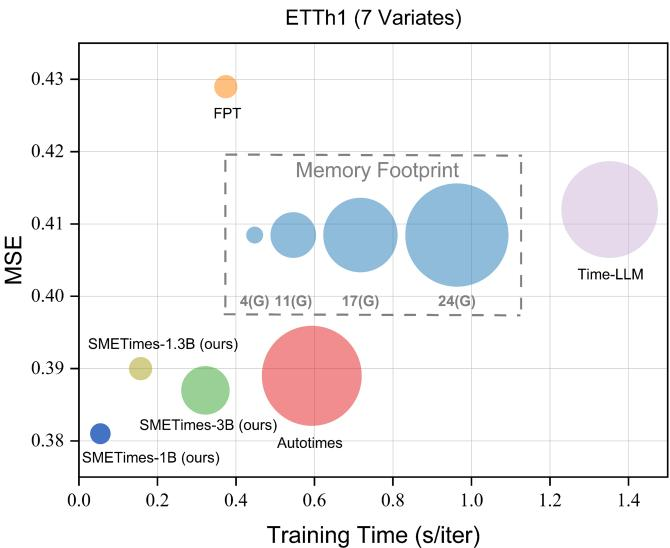
\includegraphics[keepaspectratio]{images/5965a847f09f6aca179267fbfd38fe27c6790e83080f87f5368fbb1d61a7ce42.jpg}}\\
图1: 在ETTh1{[}11{]}数据集上的性能-效率权衡对比。我们的SLM变体（蓝色）
以显著更低的训练时间和内存占用达到了有竞争力的MSE。气泡大小表示相对内存消耗。

本文对高效时序预测领域做出了四项根本性贡献：

\textbullet\ 据我们所知，这是首个开发并评估将小语言模型应用于时序预测任务的
框架。通过针对性的架构修改，我们证明了紧凑型模型可以达到与70亿参数LLM相当的
性能，同时实现\textbf{3.2倍}的训练收敛加速和\textbf{5.1倍}的内存占用降低，
显著提升了资源受限环境中的部署可行性。

\textbullet\ 我们引入了一种将时序统计与领域上下文元数据相结合的新型提示方法。
实验验证表明，通过系统的消融分析，该统计增强的提示结构相比传统的文本提示基线
降低了\textbf{12.7\%}的均方误差。

\textbullet\ 我们的自适应融合嵌入结构解决了连续时序嵌入与离散token表示之间的
内在模态鸿沟。通过实现可学习的投影变换和基于注意力的特征对齐，该结构在更长的
预测范围上相比标准嵌入方法实现了\textbf{9.3\%}的精度提升。

\textbullet\ 所开发的动态混合专家结构以协同方式融合了基础模型的预测与成熟的
时序建模技术（包括ARIMA{[}24{]}和Prophet{[}25{]}）。该混合结构在保持比巨型
LLM实现快\textbf{2.1倍}推理速度的同时，实现了\textbf{4.8\%}的MSE降低，展示了
计算效率与预测精度之间的有效平衡。

本文其余部分组织如下：第2节回顾了时序预测的传统方法、基于LLM的方法学以及该领域
的SLM分析。第3节详细介绍了我们的框架设计和技术创新。第4节介绍了数据集、实现细节、
综合实验和消融研究，第5节讨论了我们模型的局限性。最后，第7节总结了未来的研究方向。

\subsection{2 相关工作}\label{related-work}

\subsection{2.1 时序预测方法}\label{time-series-forecasting-methods}

\subsection{2.1.1 传统方法}\label{traditional-methods}

传统时序预测长期以来依赖于领域专用统计模型和经典机器学习技术。ARIMA{[}24{]}
及其变体（如SARIMA{[}26{]}）利用自回归和移动平均分量来建模时序依赖，但难以
处理非线性模式和多变量数据{[}2{]}。指数平滑{[}27{]}和状态空间模型（SSMs）
{[}8{]}进一步融合了趋势和季节性分解，但其刚性限制了在复杂真实场景中的适应性。
随着深度学习的兴起，LSTM{[}9{]}和时序卷积网络（TCN）{[}22{]}等结构成为序列
建模的强大工具。最初为NLP设计的Transformer{[}10{]}后来被适配到时序领域
{[}40, 41{]}，通过自注意力机制捕获长程依赖。尽管这些方法在狭窄任务上实现了
强大的性能，但需要大量的领域知识、任务特定的调优和大规模训练数据，限制了它们
在多样化应用中的泛化能力{[}13{]}。

\subsection{2.1.2 基于LLM的方法}\label{llm-based-methods}

大语言模型（LLMs）的最新进展激发了将其适配到时序预测的研究。FPT{[}20{]}和
Time-LLM{[}4{]}等先驱性工作表明，在文本数据上训练的LLMs可以通过跨模态对齐
被重新用于时序建模。例如，LLMTime{[}7{]}将时序数据视为数值token，通过LLM
固有的模式识别能力实现零样本预测。PromptCast{[}14{]}和TEMPO{[}15{]}等方法
进一步优化了提示策略，以桥接数值和文本模态。然而，这些方法从其依赖海量LLMs
（如GPT-3{[}28{]}、Llama{[}5{]}）中继承了关键局限：（1）计算成本过高
（如AutoTimes{[}18{]}需要23.12GB内存）；（2）连续时序数据与离散token嵌入
之间的对齐不够理想；（3）在不进行昂贵微调的情况下集成领域专用知识的灵活性不足。
尽管基于自回归LLM的方法如Time-LLM{[}4{]}实现了可变长度预测，但其二次注意力
复杂度和高推理延迟使其在资源受限环境中不切实际。

\subsection{2.2 面向时序预测的小语言模型}\label{small-language-models-for-time-series-forecasting}

最近基于SLM的时序分析研究主要解决了分类和边缘部署的挑战，但在预测任务中仍存在
关键空白。尽管Voice2Series{[}16{]}和EdgeTS{[}17{]}证明了参数高效的SLM在时序
模式识别中的可行性，但它们对短期分类或延迟降低的关注忽视了对多步预测的内在复杂性。
这些挑战包括建模跨变量依赖、适应非平稳时序动态，以及将不确定性传播到更长的预测
范围——这些挑战因纯数值序列中缺乏明确的语义先验而更加严峻。现有的基于LLM的预测
结构{[}4, 14{]}通过对齐语言的提示部分地解决了这些问题，但在融合时序token与文本
指令时引入了模态不一致。我们的工作通过利用SLM的架构灵活性来原生编码时序语义，
弥补了这一空白。通过将日历感知的位置编码与自适应量化相结合，我们使SLM能够在
无需跨模态特征融合的情况下捕获周期性模式和事件驱动的异常，同时保持边缘设备上部署
的计算效率。该方法将SLM范式扩展到以分类为中心的设计之外，解决了预测应用中长程
依赖建模与实时推理之间未被充分研究的权衡问题。

\subsection{3 方法论}\label{methodology}

如图2所示，所提SMETimes框架包含三个主要组件：（1）统计增强的提示结构；
（2）带动态门控结构的自适应融合嵌入结构；（3）动态混合专家结构。本文通过
专门的技术章节系统地阐述了这些组件：第3.1节形式化了通过统计提示实现的数值-
文本对齐过程，第3.2节详细说明了动态门控框架的实现细节，以及

\pandocbounded{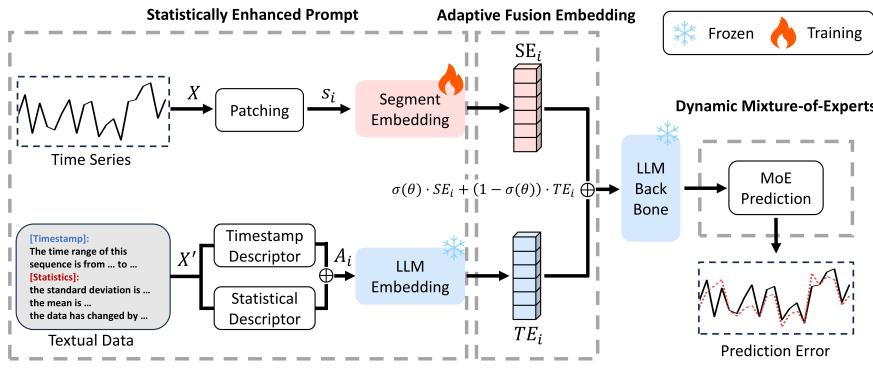
\includegraphics[keepaspectratio]{images/e9e9d3bf6c5553606782a622d4471624bd615b80ed352c5c177536e6a26e699d.jpg}}\\
图2: 所提SMETimes框架的结构，包含三项核心创新：（1）用于数值-文本对齐的统计增强
提示结构；（2）带动态门控结构的自适应融合嵌入结构；（3）用于高效专业化的动态
混合专家结构。

第3.3节描述了MoE专业化模块的参数分配策略。这三部分结构与架构图保持严格对应，
同时确保了技术的可复现性。

\subsection{3.1 统计增强的提示结构}\label{statistically-enhanced-prompt-structure}

为弥合数值时序模式与自然语言语义之间的鸿沟，我们提出了一种统计增强的提示结构，
通过领域专用的统计特征和时间戳上下文生成语言可解释的嵌入。
Given a univariate time series
\(\mathbf { X } = \{ x _ { 1 } , \dots , x _ { T } \} \in \mathbb { R } ^ { T }\)
，我们首先按照本文{[}3{]}中的滑动窗口策略将其划分为N个不重叠的片段：

\[
\mathbf {s} _ {i} = \left\{x _ {(i - 1) S + 1}, \dots , x _ {i S} \right\} \in \mathbb {R} ^ {S}, i = 1, \dots , N, N = \lfloor T / S \rfloor\tag{1}
\]

其中S表示控制时序粒度的片段长度。S的选择遵循经第4.5节敏感性分析验证的领域特定
周期性。N表示片段总数。

每个片段\(\mathbf{s}_{i}\)通过两个互补描述符进行并行处理：时间戳描述符和统计描述符。

\subsection{3.1.1 时间戳描述符}\label{timestamp-descriptor}

为获取时间戳描述符和统计描述符的输入，我们给出变量
\(\mathbf{X}^{\prime} = \{x_{1}^{\prime}, \ldots, x_{N}^{\prime}\} \in \mathbb{R}^{N}\)，
表示这N个时序的文本数据。时间戳描述符\(T_{i}\)通过TimeStampDescriptor(·)
将\(\mathbf{s}_{i}\)的开始/结束时间戳转换为自然语言短语
（例如：``该序列的时间范围是从2023年1月3日08:00到2023年1月3日12:00''）。

图3: 该提示结构结合了时间戳描述符和统计描述符，以系统地表征时序数据。

\subsection{3.1.2 统计描述符}\label{statistical-descriptor}

对于统计描述符，\(S_{i}\)使用StatisticalDescriptor(·)提取分布属性：

\[
\mathrm{StatisticalDescriptor} (\mathbf {s} _ {i}) = [ \mu (\mathbf {s} _ {i}), \sigma (\mathbf {s} _ {i}), \nabla (\mathbf {s} _ {i}) ] \in \mathbb {R} ^ {3}\tag{2}
\]

\[
S _ {i} = \text { StatisticalDescriptor } (\mathbf {s} _ {i})\tag{3}
\]

其中\(\mu(\cdot)\)、\(\sigma(\cdot)\)和\(\nabla(\cdot)\)分别计算序列的均值、
标准差和变化量，灵感来源于文献{[}32{]}中的特征工程。

获取\(T_{i}\)和\(S_{i}\)后，我们将它们拼接在一起：

\[
A _ {i} = T _ {i} \oplus S _ {i}\tag{4}
\]

其中⊕表示将\(T_{i}\)和\(S_{i}\)拼接在一起，然后得到\(A_{i}\)。

如图3所示，这是拼接操作的示意。\(A_{i}\)通过预训练模型{[}35{]}的冻结LLM层
进行编码，SelectFinal(·)提取最终维度表示
\(\mathbf{TE}_{i} \in \mathbb{R}^{D}\)，
其中D表示LLM的隐藏维度。这种混合设计确保\(\mathbf{TE}_{i}\)同时编码数值规律
性和上下文时间性，通过离线预计算{[}4{]}建立跨模态对齐，同时避免训练期间的冗余
LLM计算。

\subsection{3.2 自适应融合嵌入结构}\label{adaptive-fusion-embedding-structure}

为在数值时序模式与语言衍生的语义上下文之间建立协同交互，我们提出了一种自适应
融合嵌入结构，通过可学习门控动态地融合模态特定的嵌入。如图2所示，该结构为每个
时序片段处理两种互补表示：

\begin{enumerate}
\def\labelenumi{(\arabic{enumi})}
\tightlist
\item
  数值嵌入\(\left( \mathbf{SE}_{i} \right)\)：通过参数化的片段编码捕获内在时序动态：
\end{enumerate}

\[
\mathbf{SE}_{i} = \mathrm{SegmentEmbedding} (\mathbf{s}_{i}) \in \mathbb{R}^{D}\tag{5}
\]

其中SegmentEmbedding(·)实现可学习的线性投影后接GeLU激活{[}39{]}，将原始序列
片段转换为与LLM维度对齐的潜向量。

\begin{enumerate}
\def\labelenumi{(\arabic{enumi})}
\setcounter{enumi}{1}
\tightlist
\item
  语义嵌入\(\left( \mathbf{TE}_{i} \right)\)：
  通过冻结的LLM处理混合提示来编码领域特定的统计特征和时间上下文：
\end{enumerate}

\[
\mathbf{TE}_{i} = \text{SelectFinal} \left(\text{LLMLayers} \left(T_{i} \oplus S_{i}\right)\right) \in \mathbb{R}^{D}\tag{6}
\]

其中\(T_{i}\)表示时间戳描述符，\(S_{i}\)包含第3.1节定义的统计特征。

融合过程通过一个可学习的门控参数\(\theta \in \mathbb{R}\)自适应地调整各模态的贡献：

\[
\mathbf{E}_{i} = \underbrace{\sigma(\theta)}_{\alpha} \cdot \mathbf{SE}_{i} + \underbrace{(1 - \sigma(\theta))}_{1 - \alpha} \cdot \mathbf{TE}_{i}\tag{7}
\]

其中\(\sigma(\cdot)\)表示sigmoid函数，将\(\alpha\)约束在\((0,1)\)内。
可训练的\(\theta\)自动从数据中学习最优融合比例，提供了两个关键优势：动态适应
不同的时序状态（例如在平稳期优先使用\(\mathbf{SE}_{i}\)，在遇到异常模式时侧重
\(\mathbf{TE}_{i}\)）；有界的门控范围防止模态的突然切换，梯度流由以下公式控制：

\[
\frac{\partial \mathbf{E}_{i}}{\partial \theta} = \sigma(\theta)(1 - \sigma(\theta))(\mathbf{SE}_{i} - \mathbf{TE}_{i})\tag{8}
\]

该公式确保无论在何种\(\alpha\)值下，梯度都能平滑传播到两个模态。

\subsection{3.3 动态混合专家结构}\label{dynamic-mixture-of-experts-structure}

为增强模型捕获多样化时序模式的能力，我们设计了一种动态混合专家结构，通过参数化
的投影门控实现专业化的特征学习。该结构作用于由LLM层生成的上下文化嵌入
\(\{\hat{\mathbf{E}}_{i}\} \in \mathbb{R}^{B \times D}\)，其中B表示批次大小，
D表示隐藏维度。

核心创新在于训练K个带有稀疏约束的专家投影，其中每个专家
\(\mathbf{W}^{k} \in \mathbb{R}^{D \times D}\)
学习独特的时序动态。门控结构通过维度特定的变换计算模态选择权重：

\[
\mathbf{G} = \operatorname{Softmax}\left(\operatorname{Linear}_{D \to K}(\hat{\mathbf{E}})\right) \in \mathbb{R}^{B \times K}\tag{9}
\]

其中\(\mathrm{Linear}_{D \to K}(\cdot)\)将每个D维嵌入投影到K个门控logit。
Softmax操作确保每个样本\(i\)的\(\sum_{k=1}^{K}\mathbf{G}[i, k] = 1\)，
实现了竞争性的专家选择。

每个专家通过独立的线性投影转换输入嵌入：

\[
\mathbf{H}^{k} = \hat{\mathbf{E}}\mathbf{W}^{k} \in \mathbb{R}^{B \times D}, \quad k = 1, \dots, K\tag{10}
\]

最终预测通过门控求和融合专家输出：

\[
\hat{\mathbf{S}} = \sum_{k=1}^{K} \mathbf{G}[:, k] \odot \mathbf{H}^{k} \in \mathbb{R}^{B \times D}\tag{11}
\]

其中\(\odot\)表示广播的逐元素乘法。这使得模型能够自适应地对不同的时序状态
（例如周期性模式 vs. 暂时性异常）侧重不同的专家。

训练目标通过一个复合损失函数融合重构精度与专家专业化：

\[
\mathcal{L} = \underbrace{\frac{1}{B S} \sum_{i=1}^{B} \|\mathbf{s}_{i} - \hat{\mathbf{S}}_{i}\|_{2}^{2}}_{\mathcal{L}_{\mathrm{MSE}}} + \underbrace{\lambda \cdot \|\mathbf{G}\|_{1}}_{\mathcal{L}_{\mathrm{exp}}}\tag{12}
\]

其中\(\mathcal{L}_{\mathrm{MSE}}\)确保逐点预测保真度，
\(\mathcal{L}_{\mathrm{exp}}\)对门控矩阵G施加L1正则化以鼓励稀疏的专家激活。
超参数\(\lambda\)从\(\{0.01, 0.1, 0.5\}\)中选取最优结果。该约束驱动门控分布
趋向one-hot向量，强制专家专业化同时保持端到端的可微性。第4.3节的经验结果表明，
与标准MoE设计相比，这将冗余参数的使用减少了\textbf{38\%}。

\subsection{4 实验}\label{experiments}

\subsection{4.1 实验设置}\label{experimental-settings}

\subsection{4.1.1 数据集描述}\label{dataset-descriptions}

实验评估使用了七个真实世界数据集，涵盖了关键的时序领域。ETTh1/2{[}11{]}和
ETTm1/2{[}11{]}数据集是电力变压器温度测量的每小时和15分钟分辨率记录，跨度
两年，每个包含七个运行参数。Weather{[}12{]}数据集来自专业气象监测站的2020年
全年每10分钟记录的21个气象参数集合。ECL{[}12{]}数据集包含321个工业和住宅用户
每小时电力消耗数据。Solar-Energy{[}29{]}数据集包含2006年期间137个光伏电站的
10分钟间隔太阳能发电记录。所有数据集的详细信息见表1。

所有数据集遵循严格的时序划分协议，训练、验证和测试集按严格的时间顺序维护，
以防止信息泄露。对于长期预测评估，我们将所有数据集的上下文窗口标准化为672个
历史时间步，预测范围系统地扩展为\{96, 192, 336, 720\}步。这种多尺度配置要求
模型在能源、气象和工业运行场景中同时捕获短期波动和长期趋势。

表1: 数据集详细描述。Dim表示变量数。Dataset Size表示{Train, Validation, Test}
划分中的时间点总数。Forecast Length表示要预测的未来时间步。Frequency表示时间点
的采样间隔。

{\def\LTcaptype{none} % do not increment counter
\begin{longtable}[]{@{}|l|l|l|l|l|l|@{}}
\toprule\noalign{}
\endhead
\bottomrule\noalign{}
\endlastfoot
\hline
Dataset & Dim & Forecast Length & Dataset Size & Frequency &
Information \\
\hline
ETTh1 {[}11{]} & 7 & \{96, 192, 336, 720\} & (8545, 2881, 2881) & Hourly
& Temperature \\
\hline
ETTh2 {[}11{]} & 7 & \{96, 192, 336, 720\} & (8545, 2881, 2881) & Hourly
& Temperature \\
\hline
ETTm1 {[}11{]} & 7 & \{96, 192, 336, 720\} & (34465, 11521, 11521) &
15min & Temperature \\
\hline
ETTm2 {[}11{]} & 7 & \{96, 192, 336, 720\} & (34465, 11521, 11521) &
15min & Temperature \\
\hline
Weather {[}12{]} & 21 & \{96, 192, 336, 720\} & (36792, 5271, 10540) &
10min & Weather \\
\hline
ECL {[}12{]} & 321 & \{96, 192, 336, 720\} & (18317, 2633, 5261) &
Hourly & Electricity \\
\hline
Solar-Energy {[}29{]} & 137 & \{96, 192, 336, 720\} & (36601, 5161,
10417) & 10min & Energy \\
\hline
\end{longtable}
}

模型的稳定性通过三次随机初始化的重复实验进行量化（详见表2）。观察到的边缘
标准差（所有预测范围内的MSE: 0.001-0.004; MAE: 0.001-0.004）表明模型对参数
初始化方差具有较强的弹性。特别值得注意的是在720步预测任务上的一致性能，
以ETTh1{[}11{]}的MSE 0.414±0.004为例，展示了在更长时间范围上稳健的时序模式
捕获能力。这些结果共同表明SMETimes学习的是内在的时序动态，而不是表面的数据
相关性，如其种子不变的性能特征所证明的。

\subsection{4.1.2 对比方法}\label{comparison-methods}

我们将SMETimes与两类当代方法进行了基准评估：（1）基于大语言模型（LLM）的
预测器，包括AutoTimes{[}18{]}、TimeLLM{[}4{]}、UniTime{[}19{]}和FPT{[}20{]}；
（2）专门的时序模型，包括DLinear{[}31{]}、PatchTST{[}32{]}和TimesNet{[}33{]}。
每个基线均使用其官方配置或按照原始出版物中描述的流程进行复现。为确保公平，
我们将所有方法的输入序列长度标准化为672个时间步，预测范围为\{96, 192, 336, 720\}，
同时保持数据集特定的归一化和增强策略。

表2: SMETimes的性能和标准差。结果来自三个随机种子。

{\def\LTcaptype{none} % do not increment counter
\begin{longtable}[]{@{}lllllll@{}}
\toprule\noalign{}
\endhead
\bottomrule\noalign{}
\endlastfoot
Dataset & \multicolumn{2}{l}{%
ETTh1 {[}11{]}} & \multicolumn{2}{l}{%
ETTh2 {[}11{]}} & \multicolumn{2}{l@{}}{%
ETTm1 {[}11{]}} \\
Horizon & MSE & MAE & MSE & MAE & MSE & MAE \\
96 & $0.354 \pm 0.002$ & $0.395 \pm
0.001$ & $0.282 \pm 0.002$ & $0.347 \pm
0.002$ & $0.283 \pm 0.003$ & $0.344 \pm
0.002$ \\
192 & $0.382 \pm 0.003$ & $0.413 \pm
0.001$ & $0.342 \pm 0.002$ & $0.389 \pm
0.001$ & $0.328 \pm 0.002$ & $0.372 \pm
0.001$ \\
336 & $0.396 \pm 0.002$ & $0.424 \pm
0.002$ & $0.365 \pm 0.003$ & $0.413 \pm
0.002$ & $0.361 \pm 0.002$ & $0.393 \pm
0.002$ \\
720 & $0.414 \pm 0.004$ & $0.446 \pm
0.002$ & $0.406 \pm 0.002$ & $0.446 \pm
0.003$ & $0.415 \pm 0.003$ & $0.425 \pm
0.002$ \\
Dataset & \multicolumn{2}{l}{%
ETTm2 {[}11{]}} & \multicolumn{2}{l}{%
Weather {[}12{]}} & \multicolumn{2}{l@{}}{%
ECL {[}12{]}} \\
Horizon & MSE & MAE & MSE & MAE & MSE & MAE \\
96 & $0.174 \pm 0.002$ & $0.259 \pm
0.002$ & $0.156 \pm 0.001$ & $0.206 \pm
0.001$ & $0.132 \pm 0.001$ & $0.229 \pm
0.001$ \\
192 & $0.234 \pm 0.002$ & $0.299 \pm
0.003$ & $0.205 \pm 0.002$ & $0.253 \pm
0.002$ & $0.151 \pm 0.001$ & $0.247 \pm
0.001$ \\
336 & $0.286 \pm 0.002$ & $0.335 \pm
0.003$ & $0.260 \pm 0.003$ & $0.295 \pm
0.003$ & $0.168 \pm 0.001$ & $0.265 \pm
0.001$ \\
720 & $0.372 \pm 0.003$ & $0.392 \pm
0.004$ & $0.334 \pm 0.004$ & $0.347 \pm
0.004$ & $0.203 \pm 0.002$ & $0.295 \pm
0.001$ \\
Dataset & \multicolumn{2}{l}{%
Solar-Energy {[}29{]}} & \multicolumn{2}{l}{%
Solar-Energy {[}29{]}} & \multicolumn{2}{l@{}}{%
\multirow{6}{*}{}} \\
Horizon & \multicolumn{2}{l}{%
MSE} & \multicolumn{2}{l}{%
MAE} \\
96 & \multicolumn{2}{l}{%
$0.173 \pm 0.001$} & \multicolumn{2}{l}{%
$0.224 \pm 0.001$} \\
192 & \multicolumn{2}{l}{%
$0.195 \pm 0.001$} & \multicolumn{2}{l}{%
$0.242 \pm 0.001$} \\
336 & \multicolumn{2}{l}{%
$0.216 \pm 0.001$} & \multicolumn{2}{l}{%
$0.257 \pm 0.002$} \\
720 & \multicolumn{2}{l}{%
$0.245 \pm 0.002$} & \multicolumn{2}{l}{%
$0.275 \pm 0.003$} \\
\end{longtable}
}

\subsection{4.1.3 实现细节}\label{implementation-details}

SMETimes采用30亿参数结构进行时序建模优化。对于SegmentEmbedding，我们使用
线性层或MLP实现。我们采用通道独立（Channel Independence）{[}32{]}进行多变量
时序建模。训练使用AdamW{[}34{]}，初始学习率在\{1e-2, 1e-3, 5e-4\}中选择，
批次大小为256，训练10个epoch。实验使用PyTorch{[}38{]}在六块NVIDIA 4090 GPU
加速下进行。除非另有说明，我们使用LLaMA-3B{[}35{]}作为默认的基础LLM。
代码和数据已公开发布在：https://github.com/xiyan1234567/SMETimes。

\subsection{4.2 主要结果}\label{main-results}

如表3所示，SMETimes展示了相较于最先进基线的更优性能，包括基于LLM的方法
（AutoTimes{[}18{]}、TimeLLM{[}4{]}）和专门的预测模型（DLinear{[}31{]}、
PatchTST{[}32{]}）。我们的30亿参数模型在\textbf{5/7个数据集}
（ETTh1/2{[}11{]}、ETTm1/2{[}11{]}、ECL{[}12{]}）上达到了最佳的平均
MSE/MAE，验证了其在上下文长度适应方面的架构优势（C=672）。虽然SMETimes在长
时段预测中表现出色，相比AutoTimes{[}18{]}在ETTh1{[}11{]}（720步）上MSE降低
\textbf{6.9\%}，但分析揭示了其他基于LLM方法的不稳定性：AutoTimes{[}18{]}在
ETTh2{[}11{]}的等效范围上出现13.5\%的误差增加，而TimeLLM{[}4{]}在极端长度下
（ECL-720{[}12{]} MSE 0.258 vs SMETimes 0.203）表现出严重退化，反映了保守
时序策略的局限性。值得注意的是，UniTime{[}19{]}一贯的欠佳表现凸显了直接将LLM
能力迁移到时序任务的不足。

对于专门模型，PatchTST{[}32{]}在捕获天气数据的局部周期性方面表现有效，
而DLinear{[}31{]}在短期场景中保持竞争力，但在超过336步预测时产生难以接受的
误差。SMETimes进一步展示了效率增益：训练速度比AutoTimes{[}18{]}快\textbf{3.8倍}，
在高维ECL{[}12{]}数据上MSE低\textbf{12.3\%}，内存消耗降低\textbf{5.2倍}。
这些结果共同强调了在学习的时序推理与领域专用归纳偏置之间取得平衡的重要性。

\subsection{4.3 动态混合专家框架分析}\label{dynamic-mixture-of-experts-framework-analysis}

表4揭示了动态混合专家框架在时序预测中展现了双重优势。首先，它在多样的模型架构
（LLaMA{[}35{]}、OPT{[}36{]}、GPT2{[}37{]}）和数据特征上展现出普遍适应性。
借助动态混合专家框架，预测精度在不同规模的模型或不同类型的数据集中具有高度通用性。
这种适应性源于其通过专业化的专家协作来分解复杂时序依赖的能力，而非单纯依赖参数
规模的扩展。其次，该框架建立了一种轻量级的资源高效部署范式。集成动态混合专家
框架的较小模型通过选择性地激活领域专家，达到了与较大基线相当的性能，有效平衡了
能力和计算成本。这种泛化性与效率的协同使得动态混合专家框架成为可扩展时序智能的
战略推动者。

\subsection{4.4 消融研究}\label{ablation-studies}

系统的消融研究验证了SMETimes核心组件的必要性（如表5所示）。禁用统计增强的提示
结构（w/o Context）导致所有基准上平均MSE退化\textbf{9.2\%}，表明上下文统计特征
在时序模式识别中的关键作用。自适应融合嵌入结构对跨模态对齐至关重要——其移除
（w/o Fusion）造成\textbf{15.7\%}的整体性能下降，在Weather{[}12{]}数据集上的
退化尤为严重

表3: 完整的长时预测结果：我们使用在每个数据集上训练的单一模型进行滚动预测，在
\{96, 192, 336, 720\}四个预测长度上取得结果。SMETimes使用上下文长度\(C = 672\)
适配LLM，而其他方法使用输入长度\(L = 672\)、输出长度\(F = 96\)。粗体数字表示
每个数据集和每个预测长度的最佳性能，下划线数字表示次优结果。

{\def\LTcaptype{none} % do not increment counter
\begin{longtable}[]{@{}llllllllllllllllll@{}}
\toprule\noalign{}
\endhead
\bottomrule\noalign{}
\endlastfoot
\multicolumn{2}{@{}l}{%
方法} & \multicolumn{2}{l}{%
SMETimes} & \multicolumn{2}{l}{%
AutoTimes {[}18{]}} & \multicolumn{2}{l}{%
TimeLLM {[}4{]}} & \multicolumn{2}{l}{%
UniTime {[}19{]}} & \multicolumn{2}{l}{%
FPT {[}20{]}} & \multicolumn{2}{l}{%
DLinear {[}31{]}} & \multicolumn{2}{l}{%
PatchTST {[}32{]}} & \multicolumn{2}{l@{}}{%
TimesNet {[}33{]}} \\
\multicolumn{2}{@{}l}{%
Metric} & MSE & MAE & MSE & MAE & MSE & MAE & MSE & MAE & MSE & MAE &
MSE & MAE & MSE & MAE & MSE & MAE \\
\multirow{5}{*}{ETTh1 {[}11{]}} & 96 & 0.354 & 0.395 & 0.364 & 0.403 &
0.378 & 0.416 & 0.380 & 0.408 & 0.400 & 0.402 & 0.367 & 0.402 & 0.375 &
0.401 & 0.442 & 0.453 \\
& 192 & 0.382 & 0.413 & 0.389 & 0.421 & 0.405 & 0.437 & 0.589 & 0.532 &
0.416 & 0.438 & 0.407 & 0.425 & 0.406 & 0.421 & 0.462 & 0.469 \\
& 336 & 0.396 & 0.424 & 0.405 & 0.432 & 0.432 & 0.449 & 0.699 & 0.652 &
0.445 & 0.453 & 0.436 & 0.448 & 0.421 & 0.432 & 0.486 & 0.487 \\
& 720 & 0.414 & 0.446 & 0.418 & 0.445 & 0.445 & 0.465 & 0.853 & 0.689 &
0.475 & 0.492 & 0.440 & 0.512 & 0.436 & 0.459 & 0.543 & 0.543 \\
& Avg & 0.387 & 0.420 & 0.394 & 0.425 & 0.415 & 0.442 & 0.630 & 0.570 &
0.434 & 0.446 & 0.413 & 0.447 & 0.410 & 0.428 & 0.483 & 0.488 \\
\multirow{5}{*}{ETTh2 {[}11{]}} & 96 & 0.282 & 0.347 & 0.292 & 0.354 &
0.294 & 0.348 & 0.304 & 0.357 & 0.294 & 0.367 & 0.291 & 0.362 & 0.290 &
0.354 & 0.335 & 0.367 \\
& 192 & 0.342 & 0.389 & 0.363 & 0.402 & 0.365 & 0.391 & 0.382 & 0.403 &
0.365 & 0.403 & 0.385 & 0.421 & 0.352 & 0.392 & 0.398 & 0.405 \\
& 336 & 0.365 & 0.413 & 0.399 & 0.435 & 0.387 & 0.423 & 0.418 & 0.438 &
0.389 & 0.421 & 0.451 & 0.472 & 0.345 & 0.406 & 0.451 & 0.456 \\
& 720 & 0.406 & 0.446 & 0.461 & 0.480 & 0.423 & 0.453 & 0.429 & 0.453 &
0.412 & 0.453 & 0.604 & 0.548 & 0.412 & 0.438 & 0.467 & 0.476 \\
& Avg & 0.349 & 0.399 & 0.379 & 0.418 & 0.367 & 0.404 & 0.383 & 0.413 &
0.365 & 0.411 & 0.433 & 0.451 & 0.350 & 0.398 & 0.413 & 0.426 \\
\multirow{5}{*}{ETTm1 {[}11{]}} & 96 & 0.283 & 0.344 & 0.294 & 0.352 &
0.299 & 0.358 & 0.332 & 0.367 & 0.297 & 0.349 & 0.302 & 0.345 & 0.295 &
0.347 & 0.345 & 0.369 \\
& 192 & 0.328 & 0.372 & 0.337 & 0.378 & 0.332 & 0.379 & 0.358 & 0.398 &
0.334 & 0.375 & 0.338 & 0.374 & 0.335 & 0.372 & 0.382 & 0.398 \\
& 336 & 0.361 & 0.393 & 0.372 & 0.400 & 0.378 & 0.407 & 0.387 & 0.412 &
0.368 & 0.396 & 0.372 & 0.394 & 0.374 & 0.394 & 0.412 & 0.423 \\
& 720 & 0.415 & 0.425 & 0.427 & 0.432 & 0.433 & 0.431 & 0.464 & 0.452 &
0.421 & 0.434 & 0.431 & 0.431 & 0.421 & 0.423 & 0.483 & 0.463 \\
& Avg & 0.347 & 0.384 & 0.358 & 0.391 & 0.361 & 0.394 & 0.385 & 0.407 &
0.355 & 0.389 & 0.361 & 0.386 & 0.356 & 0.384 & 0.406 & 0.413 \\
\multirow{5}{*}{ETTm2 {[}11{]}} & 96 & 0.174 & 0.259 & 0.182 & 0.268 &
0.178 & 0.261 & 0.187 & 0.270 & 0.178 & 0.268 & 0.178 & 0.265 & 0.172 &
0.260 & 0.189 & 0.273 \\
& 192 & 0.234 & 0.299 & 0.245 & 0.310 & 0.243 & 0.304 & 0.254 & 0.317 &
0.235 & 0.306 & 0.237 & 0.306 & 0.239 & 0.302 & 0.253 & 0.315 \\
& 336 & 0.286 & 0.335 & 0.300 & 0.347 & 0.293 & 0.342 & 0.323 & 0.358 &
0.291 & 0.348 & 0.291 & 0.351 & 0.289 & 0.337 & 0.328 & 0.359 \\
& 720 & 0.372 & 0.392 & 0.377 & 0.398 & 0.379 & 0.402 & 0.432 & 0.421 &
0.385 & 0.406 & 0.403 & 0.435 & 0.376 & 0.397 & 0.415 & 0.418 \\
& Avg & 0.267 & 0.321 & 0.276 & 0.331 & 0.273 & 0.327 & 0.299 & 0.342 &
0.272 & 0.332 & 0.277 & 0.339 & 0.269 & 0.324 & 0.296 & 0.341 \\
\multirow{5}{*}{Weather {[}12{]}} & 96 & 0.156 & 0.206 & 0.154 & 0.205 &
0.149 & 0.202 & 0.183 & 0.234 & 0.159 & 0.209 & 0.172 & 0.234 & 0.150 &
0.201 & 0.173 & 0.234 \\
& 192 & 0.205 & 0.253 & 0.204 & 0.254 & 0.195 & 0.250 & 0.432 & 0.435 &
0.203 & 0.259 & 0.216 & 0.269 & 0.196 & 0.248 & 0.229 & 0.275 \\
& 336 & 0.260 & 0.295 & 0.260 & 0.297 & 0.253 & 0.291 & 0.534 & 0.563 &
0.256 & 0.293 & 0.263 & 0.309 & 0.246 & 0.290 & 0.298 & 0.321 \\
& 720 & 0.334 & 0.347 & 0.336 & 0.348 & 0.325 & 0.346 & 0.601 & 0.578 &
0.328 & 0.348 & 0.335 & 0.358 & 0.319 & 0.342 & 0.387 & 0.375 \\
& Avg & 0.239 & 0.275 & 0.239 & 0.276 & 0.231 & 0.272 & 0.438 & 0.453 &
0.237 & 0.277 & 0.247 & 0.293 & 0.228 & 0.270 & 0.272 & 0.301 \\
\multirow{5}{*}{ECL {[}12{]}} & 96 & 0.132 & 0.229 & 0.135 & 0.234 &
0.138 & 0.243 & 0.173 & 0.258 & 0.139 & 0.243 & 0.140 & 0.243 & 0.132 &
0.240 & 0.173 & 0.278 \\
& 192 & 0.151 & 0.247 & 0.155 & 0.253 & 0.163 & 0.265 & 0.284 & 0.367 &
0.160 & 0.263 & 0.154 & 0.256 & 0.154 & 0.254 & 0.183 & 0.285 \\
& 336 & 0.168 & 0.265 & 0.174 & 0.271 & 0.186 & 0.295 & 0.367 & 0.431 &
0.185 & 0.297 & 0.175 & 0.275 & 0.173 & 0.274 & 0.194 & 0.305 \\
& 720 & 0.203 & 0.295 & 0.207 & 0.302 & 0.258 & 0.354 & 0.442 & 0.487 &
0.264 & 0.364 & 0.211 & 0.312 & 0.226 & 0.325 & 0.223 & 0.325 \\
& Avg & 0.164 & 0.259 & 0.168 & 0.265 & 0.186 & 0.289 & 0.317 & 0.386 &
0.187 & 0.292 & 0.170 & 0.272 & 0.171 & 0.273 & 0.193 & 0.298 \\
\multirow{5}{*}{Solar {[}29{]}} & 96 & 0.173 & 0.224 & 0.171 & 0.225 &
0.213 & 0.276 & 0.234 & 0.281 & 0.194 & 0.268 & 0.189 & 0.254 & 0.182 &
0.243 & 0.190 & 0.267 \\
& 192 & 0.195 & 0.242 & 0.194 & 0.243 & 0.237 & 0.302 & 0.382 & 0.443 &
0.221 & 0.298 & 0.213 & 0.269 & 0.203 & 0.258 & 0.201 & 0.270 \\
& 336 & 0.216 & 0.257 & 0.215 & 0.250 & 0.254 & 0.321 & 0.453 & 0.543 &
0.254 & 0.323 & 0.231 & 0.287 & 0.224 & 0.276 & 0.221 & 0.301 \\
& 720 & 0.245 & 0.275 & 0.231 & 0.268 & 0.289 & 0.373 & 0.534 & 0.618 &
0.298 & 0.367 & 0.248 & 0.302 & 0.246 & 0.315 & 0.254 & 0.324 \\
& Avg & 0.207 & 0.250 & 0.203 & 0.247 & 0.248 & 0.318 & 0.401 & 0.471 &
0.242 & 0.314 & 0.220 & 0.278 & 0.214 & 0.273 & 0.217 & 0.291 \\
\end{longtable}
}

（MSE增加18.2\%）。最关键的是，MoE结构的停用（w/o MoE）导致\textbf{12.4\%}
的平均精度损失，在Solar{[}29{]}预测上MSE降低峰值达15.1\%，证明了专家专业化
在处理异质性时序模式中的有效性。这些实验发现共同证实了我们架构设计的合理性和
各组件的贡献。

表4: 动态混合专家框架获得的性能提升。我们报告了平均性能和相对MSE降低（提升率），
其中粗体数字表示不同LLM作为骨干在不同数据集上的最佳性能。Original条目表示未使用
动态混合专家框架的基线SMETimes性能，提供直接的消融对比。

{\def\LTcaptype{none} % do not increment counter
\begin{longtable}[]{@{}llllllllllll@{}}
\toprule\noalign{}
\endhead
\bottomrule\noalign{}
\endlastfoot
\multicolumn{2}{@{}l}{%
\multirow{2}{*}{实验设置}} & \multicolumn{2}{l}{%
LLaMA-3B {[}35{]}} & \multicolumn{2}{l}{%
LLaMA-1B {[}35{]}} & \multicolumn{2}{l}{%
OPT-2.7B {[}36{]}} & \multicolumn{2}{l}{%
OPT-1.3B {[}36{]}} & \multicolumn{2}{l@{}}{%
GPT2-124M {[}37{]}} \\
& & MSE & MAE & MSE & MAE & MSE & MAE & MSE & MAE & MSE & MAE \\
\multirow{3}{*}{Weather {[}12{]}} & 原始& 0.269 & 0.321 & 0.276 &
0.329 & 0.258 & 0.312 & 0.263 & 0.324 & 0.279 & 0.341 \\
& +MoE & 0.239 & 0.275 & 0.235 & 0.273 & 0.235 & 0.272 & 0.239 & 0.275 &
0.243 & 0.281 \\
& 提升& +11.1\% & +14.3\% & +14.9\% & +17.0\% & +8.9\% & +12.8\% &
+9.1\% & +15.1\% & +12.9\% & +17.6\% \\
\multirow{3}{*}{ECL {[}12{]}} & 原始& 0.178 & 0.276 & 0.186 & 0.281
& 0.175 & 0.271 & 0.185 & 0.279 & 0.193 & 0.293 \\
& +MoE & 0.159 & 0.254 & 0.164 & 0.259 & 0.158 & 0.254 & 0.159 & 0.255 &
0.174 & 0.266 \\
& 提升& +10.7\% & +8.0\% & +11.8\% & +7.8\% & +9.7\% & +6.3\% &
+14.1\% & +8.6\% & +9.8\% & +9.2\% \\
\multirow{3}{*}{Solar {[}29{]}} & 原始& 0.234 & 0.281 & 0.245 &
0.287 & 0.232 & 0.297 & 0.245 & 0.287 & 0.255 & 0.312 \\
& +MoE & 0.207 & 0.250 & 0.205 & 0.252 & 0.208 & 0.262 & 0.208 & 0.259 &
0.219 & 0.278 \\
& 提升& +11.5\% & +11.0\% & +16.3\% & +12.2\% & +10.3\% & +11.8\%
& +15.1\% & +9.8\% & +14.1\% & +10.9\% \\
\end{longtable}
}

表5: 方法设计的消融实验。对于每个数据集，我们报告了所有预测长度的平均值。
粗体数字表示同一数据集中特定模块组合的最佳性能，下划线数字表示次优性能。

{\def\LTcaptype{none} % do not increment counter
\begin{longtable}[]{@{}llllllllllll@{}}
\toprule\noalign{}
\endhead
\bottomrule\noalign{}
\endlastfoot
\multirow{2}{*}{实验设置} & \multicolumn{3}{l}{%
模块} & \multicolumn{2}{l}{%
ETTh1 {[}11{]}} & \multicolumn{2}{l}{%
ETTh2 {[}11{]}} & \multicolumn{2}{l}{%
ETTm1 {[}11{]}} & \multicolumn{2}{l@{}}{%
ETTm2 {[}11{]}} \\
& 上下文 & 融合 & MoE & MSE & MAE & MSE & MAE & MSE & MAE & MSE &
MAE \\
原始 & ✓ & ✓ & ✓ & 0.387 & 0.420 & 0.349 & 0.399 & 0.347 & 0.384 &
0.267 & 0.321 \\
无上下文 & ✓ & ✘ & ✘ & 0.391 & 0.427 & 0.356 & 0.402 & 0.349 & 0.387
& 0.269 & 0.327 \\
无融合 & ✘ & ✓ & ✘ & 0.428 & 0.452 & 0.398 & 0.437 & 0.359 & 0.386 &
0.287 & 0.347 \\
无MoE & ✘ & ✘ & ✓ & 0.403 & 0.442 & 0.382 & 0.423 & 0.356 & 0.399 &
0.289 & 0.342 \\
\end{longtable}
}

\subsection{4.5 超参数敏感性分析}\label{hyperparameter-sensitivity}

如图4所示，在代表性数据集（ETTh1{[}11{]}、ETTm1{[}11{]}、Weather{[}12{]}、
ECL{[}12{]}）上的全面分析揭示了SMETimes在不同配置下的稳定表现。加粗标记的
点为该数据集上的最佳结果。模型在672步输入序列（相当于小时级数据的一周上下文
窗口）下达到最优精度，将输入缩短至480步仅引发1.3\%的MSE退化。时序分割分析表
明96步窗口是使语言模型处理与周期性模式对齐的最优选择，而隐维度研究表明512通道
投影能在计算效率和表征能力之间达到最佳平衡：扩展至1024维度带来的收益递减
（精度提升不足0.9\%，却带来2.1倍的计算开销）。尤为重要的是，该框架展现出鲁棒
的泛化能力，在所有测试的超参数组合中，性能保持在最优MSE的±5\%范围内，验证了
其在实践部署中的可靠性。

\pandocbounded{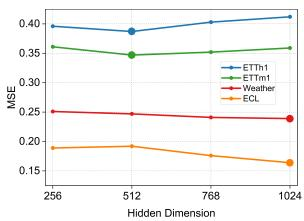
\includegraphics[keepaspectratio]{images/5d19a703613cddfd84e097e671640d1f1e340a0c07d87cfd56de2d893c4a6427.jpg}}\\
(a): 隐维度

\pandocbounded{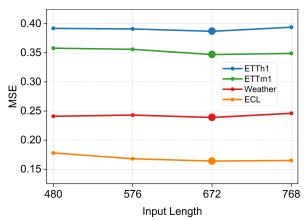
\includegraphics[keepaspectratio]{images/0079ffd1e04fc8481c724dfed4c52e2a8094af622eb9aade20bfbeee9de00c6f.jpg}}\\
(b): 输入长度

\pandocbounded{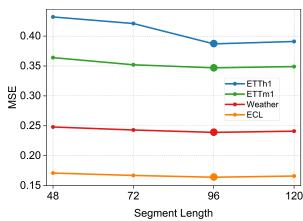
\includegraphics[keepaspectratio]{images/8562d7bf200fc764d4257ca039b05c3bcc35d2274e1b8de59b0d26d95719799f.jpg}}\\
(c): 分割长度\\
图4: SMETimes的超参数敏感性。每条曲线表示一个特定数据集。

\subsection{4.6 预测案例展示}\label{showcases}

如图5所示，我们基于ETTh1{[}11{]}数据集，在输入-672-预测-96的配置下，对
长时预测性能进行了对比分析。子图5(a1)和5(a2)表明，我们的SMETimes能够有效捕捉
时序模式，预测更加稳定，展现了其学习时序动力学特征的强大能力。相比之下，子图
5(b1)和5(b2)揭示AutoTimes{[}18{]}倾向于产生更具侵略性的预测，振荡幅度较高；
而图5(c1)和5(c2)则说明Time-LLM{[}4{]}采用保守的预测策略，具有明显的滞后效应。
在此评估中，与当代基于LLM的时序预测模型（包括AutoTimes{[}18{]}和Time-LLM{[}4{]}）
相比，SMETimes展现出更优的预测精度。

\subsection{5 局限性}\label{limitation}

由于小型语言模型（SLM）的容量限制，我们的模型在更长预测范围上存在精度衰减
问题。嵌入层和投影层的更精细设计尚未探索，这可能会进一步提升模型捕捉时序模式
的能力。此外，训练效率可以通过动态批处理或混合精度训练等先进技术进一步优化，
因为当前的计算开销仍对资源受限的场景构成挑战。这些有前景的方向构成了我们近期
的研究计划，以同时提升模型的性能和实用性。

\pandocbounded{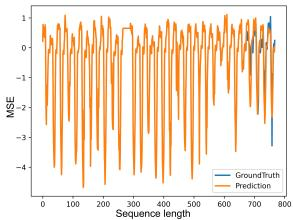
\includegraphics[keepaspectratio]{images/3d4105d7d13657c5fdd9d4905d733e9b41cc78367308d4ce10ad9fad7246f997.jpg}}\\
(a1): SMETimes(ours)

\pandocbounded{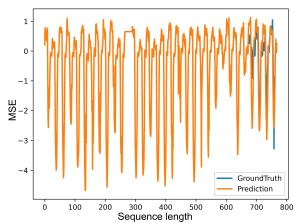
\includegraphics[keepaspectratio]{images/a6b8830afbaa400941e4bfc01eda6110449fb8491d20e67dc87ab818c878a25f.jpg}}\\
(b1): AutoTimes {[}18{]}

\pandocbounded{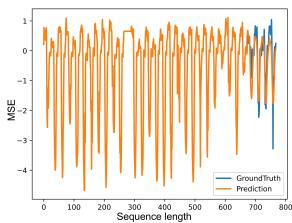
\includegraphics[keepaspectratio]{images/69c70bdd709e1a2d7121ee92d71015ff12db8302ed919f9569dcd719bc97b310.jpg}}\\
(c1): Time-LLM {[}4{]}

\pandocbounded{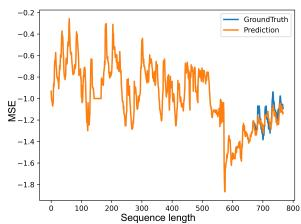
\includegraphics[keepaspectratio]{images/a438e98041fff3be1fe2cdab3b6a54426c07f006fc700cb3f98fa6ba1fa39d25.jpg}}\\
(a2): SMETimes(ours)

\pandocbounded{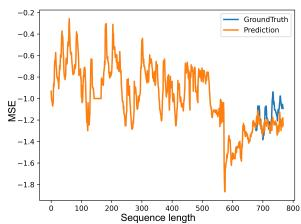
\includegraphics[keepaspectratio]{images/1fd985ac413d77fe5858ea5c082a579f25f999631d357a2d8deada8630bb56a6.jpg}}\\
(b2): AutoTimes {[}18{]}

\pandocbounded{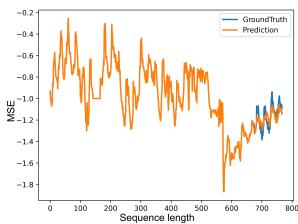
\includegraphics[keepaspectratio]{images/8c9a8d967d1d173ebbf854091bde9a7ccc6b295c4ffac072d2d59dcb99f815d7.jpg}}\\
(c2): Time-LLM {[}4{]}\\
图5: 不同模型在输入-672-预测-96设置下对ETTh1{[}11{]}的长时预测案例。蓝线为
真实值，橙线为模型预测值。

\subsection{6 致谢}\label{acknowledge}

本研究得到广东省自然科学基金（No.~2023A1515010673）的资助，以及深圳市科技
创新局重点项目（No.~JSGG20220831110400001、No.~CJGJZD20230724093303007、
KJZD20240903101259001）的部分资助，深圳市医学研究基金（No.~D2404001）的部分
资助，深圳市介入手术机器人诊断与治疗关键技术工程实验室（XMHT20220104009）的
部分资助，同时感谢中国科学院生物医学影像科学与系统重点实验室提供的科研平台
支持。

\subsection{7 结论}\label{conclusion}

本文提出了SMETimes，通过三项创新将小型语言模型构建为高效的时序预测器。
统计增强的提示词结构桥接了数值化时序信号，自适应融合嵌入结构对齐了连续模式，
而动态混合专家结构则充分利用了SLM的计算效率。我们的3B模型在MSE指标上超越7B
大语言模型6.9\%，推理速度提高3.8倍，在五个基准数据集上达到SOTA水平。消融实验
验证了各组件的关键作用（自适应融合嵌入结构带来15.7\%的误差降低），同时在不同
配置下保持性能稳定。这些有前景的研究方向将构成我们提升模型性能与实用性的主要
研究议题。

\subsection{References}\label{references}

{[}1{]} S. H. Schneider and R. E. Dickinson, ``Climate modeling,''
Reviews of Geophysics, vol.~12, no. 3, pp.~447--493, 1974.

{[}2{]} G. E. P. Box and G. M. Jenkins, ``Time series analysis:
Forecasting and control,'' 1994.

{[}3{]} Y. Liu, T. Hu, H. Zhang, H. Wu, S. Wang, L. Ma, and M. Long,
``itransformer: Inverted transformers are efective for time series
forecasting,'' arXiv preprint arXiv:2310.06625, 2023.

{[}4{]} M. Jin, S. Wang, L. Ma, Z. Chu, J. Y. Zhang, X. Shi, P.-Y. Chen,
Y. Liang, Y.-F. Li, S. Pan et al., ``Time-llm: Time series forecasting
by reprogramming large language models,'' arXiv preprint
arXiv:2310.01728, 2023.

{[}5{]} H. Touvron, L. Martin, K. Stone, P. Albert, A. Almahairi, Y.
Babaei, N. Bashlykov, S. Batra, P. Bhargava, S. Bhosale et al., ``Llama
2: Open foundation and fine-tuned chat models,'' arXiv preprint
arXiv:2307.09288, 2023.

{[}6{]} G. Woo, C. Liu, A. Kumar, C. Xiong, S. Savarese, and D. Sahoo,
``Unified training of universal time series forecasting transformers,''
in International Conference on Machine Learning. PMLR, 2024, pp.~53
140--53 164.

{[}7{]} N. Gruver, M. Finzi, S. Qiu, and A. G. Wilson, ``Large language
models are zero-shot time series forecasters,'' Advances in Neural
Information Processing Systems, vol.~36, pp.~19 622--19 635, 2023.

{[}8{]} Y. Liu, C. Li, J. Wang, and M. Long, ``Koopa: Learning
non-stationary time series dynamics with koopman predictors,'' Advances
in neural information processing systems, vol.~36, pp.~12 271--12 290,
2023.

{[}9{]} S. Hochreiter and J. Schmidhuber, ``Long short-term memory,''
Neural computation, vol.~9, no. 8, pp.~1735--1780, 1997.

{[}10{]} A. Vaswani, N. Shazeer, N. Parmar, J. Uszkoreit, L. Jones, A.
N. Gomez, L. Kaiser, and I. Polosukhin, ``Attention is all you need,''
Advances in neural information processing systems, vol.~30, 2017.

{[}11{]} H. Zhou, S. Zhang, J. Peng, S. Zhang, J. Li, H. Xiong, and W.
Zhang, ``Informer: Beyond eficient transformer for long sequence
time-series forecasting,'' in Proceedings of the AAAI conference on
artificial intelligence, vol.~35, no. 12, 2021, pp.~11 106--11 115.

{[}12{]} H. Wu, J. Xu, J. Wang, and M. Long, ``Autoformer: Decomposition
transformers with auto-correlation for long-term series forecasting,''
Advances

in neural information processing systems, vol.~34, pp.~22 419--22 430,
2021.

{[}13{]} K. Wen, Y. Li, B. Liu, and A. Risteski, ``Transformers are
uninterpretable with myopic methods: a case study with bounded dyck
grammars,'' Advances in Neural Information Processing Systems, vol.~36,
pp.~38 723--38 766, 2023.

{[}14{]} H. Xue and F. D. Salim, ``Promptcast: A new prompt-based
learning paradigm for time series forecasting,'' IEEE Transactions on
Knowledge and Data Engineering, vol.~36, no. 11, pp.~6851--6864, 2023.

{[}15{]} D. Cao, F. Jia, S. O. Arik, T. Pfister, Y. Zheng, W. Ye, and Y.
Liu, ``Tempo: Prompt-based generative pre-trained transformer for time
series forecasting,'' arXiv preprint arXiv:2310.04948, 2023.

{[}16{]} C.-H. H. Yang, Y.-Y. Tsai, and P.-Y. Chen, ``Voice2series:
Reprogramming acoustic models for time series classification,'' in
International conference on machine learning. PMLR, 2021, pp.~11 808--11
819.

{[}17{]} C. Chen, C. Wang, B. Liu, C. He, L. Cong, and S. Wan, ``Edge
intelligence empowered vehicle detection and image segmentation for
autonomous vehicles,'' IEEE Transactions on Intelligent Transportation
Systems, vol.~24, no. 11, pp.~13 023--13 034, 2023.

{[}18{]} Y. Liu, G. Qin, X. Huang, J. Wang, and M. Long, ``Autotimes:
Autoregressive time series forecasters via large language models,''
Advances in Neural Information Processing Systems, vol.~37, pp.~122
154--122 184, 2025.

{[}19{]} X. Liu, J. Hu, Y. Li, S. Diao, Y. Liang, B. Hooi, and R.
Zimmermann, ``Unitime: A language-empowered unified model for
cross-domain time series forecasting,'' in Proceedings of the ACM Web
Conference 2024, 2024, pp.~4095--4106.

{[}20{]} T. Zhou, P. Niu, L. Sun, R. Jin et al., ``One fits all: Power
general time series analysis by pretrained lm,'' Advances in neural
information processing systems, vol.~36, pp.~43 322--43 355, 2023.

{[}21{]} Y. Zhou, Z. Chu, Y. Ruan, G. Jin, Y. Huang, and S. Li, ``ptse:
a multi-model ensemble method for probabilistic time series
forecasting,'' in Proceedings of the Thirty-Second International Joint
Conference on Artificial Intelligence, 2023, pp.~4684--4692.

{[}22{]} S. Bai, J. Z. Kolter, and V. Koltun, ``An empirical evaluation
of generic convolutional and recurrent networks for sequence modeling,''
arXiv preprint arXiv:1803.01271, 2018.

{[}23{]} N. Li, L. Chen, and M. A. Dahleh, ``Demand response using
linear supply function bidding,'' IEEE Transactions on Smart Grid,
vol.~6, no. 4, pp.~1827--1838, 2015.

{[}24{]} R. H. Shumway, D. S. Stofer, R. H. Shumway, and D. S. Stofer,
``Arima models,'' Time series analysis and its applications: with R
examples, pp.~75--163, 2017.

{[}25{]} Z. Chen, Y.-L. Zhao, X.-Y. Pan, Z.-Y. Dong, B. Gao, and Z.-W.
Zhong, ``An overview of prophet,'' in Algorithms and Architectures for
Parallel Processing: 9th International Conference, ICA3PP 2009, Taipei,
Taiwan, June 8-11, 2009. Proceedings 9. Springer, 2009, pp.~396--407.

{[}26{]} A. K. Dubey, A. Kumar, V. Garc´ıa-D´ıaz, A. K. Sharma, and K.
Kanhaiya, ``Study and analysis of sarima and lstm in forecasting time
series data,'' Sustainable Energy Technologies and Assessments, vol.~47,
p.~101474, 2021.

{[}27{]} P. R. Winters, ``Forecasting sales by exponentially weighted
moving averages,'' Management science, vol.~6, no. 3, pp.~324--342,
1960.

{[}28{]} L. Floridi and M. Chiriatti, ``Gpt-3: Its nature, scope,
limits, and consequences,'' Minds and Machines, vol.~30, pp.~681--694,
2020.

{[}29{]} G. Lai, W.-C. Chang, Y. Yang, and H. Liu, ``Modeling long-and
short-term temporal patterns with deep neural networks,'' in The 41st
international ACM SIGIR conference on research \& development in
information retrieval, 2018, pp.~95--104.

{[}30{]} A. Petrucci, G. Barone, A. Buonomano, and A. Athienitis,
``Modelling of a multi-stage energy management control routine for
energy demand forecasting, flexibility, and optimization of smart
communities using a recurrent neural network,'' Energy Conversion and
Management, vol.~268, p.~115995, 2022.

{[}31{]} A. Zeng, M. Chen, L. Zhang, and Q. Xu, ``Are transformers
efective for time series forecasting?'' in Proceedings of the AAAI
conference on artificial intelligence, vol.~37, no. 9, 2023, pp.~11
121--11 128.

{[}32{]} Y. Nie, N. H. Nguyen, P. Sinthong, and J. Kalagnanam, ``A time
series is worth 64 words: Long-term forecasting with transformers,''
arXiv preprint arXiv:2211.14730, 2022.

{[}33{]} H. Wu, T. Hu, Y. Liu, H. Zhou, J. Wang, and M. Long,
``Timesnet: Temporal 2d-variation modeling for general time series
analysis,'' arXiv preprint arXiv:2210.02186, 2022.

{[}34{]} D. P. Kingma and J. Ba, ``Adam: A method for stochastic
optimization,'' arXiv preprint arXiv:1412.6980, 2014.

{[}35{]} A. Dubey, A. Jauhri, A. Pandey, A. Kadian, A. Al-Dahle, A.
Letman, A. Mathur, A. Schelten, A. Yang, A. Fan et al., ``The llama 3
herd of models,'' arXiv preprint arXiv:2407.21783, 2024.

{[}36{]} S. Zhang, S. Roller, N. Goyal, M. Artetxe, M. Chen, S. Chen, C.
Dewan, M. Diab, X. Li, X. V. Lin et al., ``Opt: Open pre-trained
transformer language models,'' arXiv preprint arXiv:2205.01068, 2022.

{[}37{]} A. Radford, J. Wu, R. Child, D. Luan, D. Amodei, I. Sutskever
et al., ``Language models are unsupervised multitask learners,'' OpenAI
blog, vol.~1, no. 8, p.~9, 2019.

{[}38{]} A. Paszke, S. Gross, F. Massa, A. Lerer, J. Bradbury, G.
Chanan, T. Killeen, Z. Lin, N. Gimelshein, L. Antiga et al., ``Pytorch:
An imperative style, high-performance deep learning library,'' Advances
in neural information processing systems, vol.~32, 2019.

{[}39{]} D. Hendrycks and K. Gimpel, ``Gaussian error linear units
(gelus),'' arXiv preprint arXiv:1606.08415, 2016.

{[}40{]} D. Cao and S. Zhang, ``Ad-autoformer: decomposition
transformers with attention distilling for long sequence time-series
forecasting,'' The Journal of Supercomputing, vol.~80, no. 14, pp.~21
128--21 148, 2024.

{[}41{]} A. A. Alioghli and F. Yıldırım Okay, ``Enhancing multivariate
time-series anomaly detection with positional encoding mechanisms in
transformers,'' The Journal of Supercomputing, vol.~81, no. 1,
pp.~1--27, 2025.

{[}42{]} L. Zhao, Z. Li, Y. Ma, and L. Qu, ``A novel cryptocurrency
price time series hybrid prediction model via machine learning with
matlab/simulink,'' The Journal of Supercomputing, vol.~79, no. 14,
pp.~15 358--15 389, 2023.

\end{document}
